\documentclass[11pt]{article}
\usepackage{amssymb,graphicx,amsmath,mathtools,float}
\usepackage{lscape}
\usepackage[utf8]{inputenc}
\usepackage[spanish, es-tabla]{babel}

\usepackage{indentfirst}	% Tabular tras un section
\usepackage{hyperref}
\hypersetup{
	colorlinks=false,
	citecolor=black,
	filecolor=black,
	linkcolor=red,
	urlcolor=black,
	pdfborderstyle={/S/U/W 1}
}

\usepackage[svgnames]{xcolor}
\definecolor{griscaption}{RGB}{100,100,100}
\usepackage{caption}
\usepackage[font={color=griscaption},figurename=Fig.,labelfont={bf}]{caption}


\newtheorem{theorem}{Theorem}
\newtheorem{corollary}[theorem]{Corollary}
\newtheorem{lemma}[theorem]{Lemma}
\newtheorem{proposition}[theorem]{Proposition}
\newtheorem{definition}[theorem]{Definición}


\title{Determinación de Órbitas Elípticas}
\author{Simón López
\\
{\small Matemáticas e Ingeniería Informática}
\\
{\small Universidad de Granada, 18071 Granada, Spain}
\\
{\small simondelosbros@correo.ugr.es}}
\date{\today}
\setlength{\unitlength}{1cm}
\setlength{\unitlength}{1cm}


\begin{document}
\maketitle

\section{Introducción}

El problema de determinación de órbitas consiste en determinar los elementos orbitales de un cuerpo observado a partir de $N$ observaciones con un grado de exactitud requerido. La dificultad surge del hecho de que una observación realizada desde la Tierra, la cuál se encuentra en continuo movimiento, nos proporcionará la dirección del cuerpo percibida por el observador, sin ninguna información sobre su distancia. Al no disponer de esta distancia no podremos determinar su posición exacta y las componentes de la velocidad no podrán ser determinadas. Así, habremos de disponer de observaciones complementarias. Pero, ¿cuántas necesitaremos, como poco, para obtener todos los elementos de la órbita?\\

A lo largo de esta memoria veremos que una órbita se define por seis elementos, por lo que nos bastará con que las observaciones nos proporcionen al menos seis valores independientes entre ellos. A partir de una observación completa (\textit{podría hablar sobre métodos de observación en un anexo}) obtenemos dos cantidades, referentes a las coordenadas angulares del cuerpo observado; por lo tanto, serán suficientes tres observaciones del objeto a determinar su órbita para comenzar nuestro proceso. Por otra parte, tener en cuenta que, previo a nuestro estudio, podemos conocer algunos elementos de la órbita; por ejemplo, si la órbita es parabólica, conocemos su excentricidad ($e=1$), por lo que no serán necesarios seis elementos, sino cinco, y de esta manera una de las observaciones realizada puede ser dejada a medias, proporcionando solo una de las coordenadas angulares.\\

Las coordenadas angulares del cuerpo que observemos serán obtenidas en ascensión recta y declinación, ya que la posición del cuerpo será determinada midiendo las distancias angulares y direcciones respecto a las estrellas vecinas, que están catalogadas en este tipo de coordenadas. Aún así, podremos cambiar a cualquier otro tipo de sistema de coordenadas en cuando queramos.\\

Comencemos viendo cuáles son los distintos elementos de una órbita, así como qué es la ascensión recta y declinación, que en conjunto llamaremos coordenadas ecuatoriales.\\


\section{Elementos Orbitales y Coordenadas Ecuatoriales}
En esta sección estudiaremos los diferentes parámetros que identifican una órbita (de manera única) así como las coordenadas ecuatoriales, elementos que forman un sistema que nos permite ubicar el objeto observado respecto al \textit{ecuador celeste} y al \textit{equinoccio vernal}, que definiremos más adelante, en un momento preciso.\\

\subsection{Elementos Orbitales}
Comencemos por los elementos orbitales, los cuales necesitarán sostenerse en las dos primeras leyes de Kepler para ser desarrollados	. Dichas leyes son:

\begin{enumerate}
\item \textit{Todos los planetas se desplazan alrededor del Sol describiendo órbitas elípticas, con el Sol en uno de los focos de dicha elipse.}
\item \textit{Cada objeto barre áreas iguales en tiempos iguales.}
\end{enumerate}

Pues bien, con esto comencemos a desarrollar nuestros elementos entendiendo qué es una elipse y como se comporta matemáticamente.\\

\begin{definition}
La elipse es una curva plana, simple y cerrada, que consta de dos focos (puntos fijos) de manera que para cualquier punto de la curva que tomemos, la suma de las distancias de los focos a dicho punto es la misma.
\end{definition}

Llamando a nuestra elipse $E$ y a los focos de ésta $F_1$ y $F_2$, podemos escribir las definición de la siguiente manera:
\[
|x-F_1|+|x-F_2|=d, \; \forall x \in E \implies d>|F_1-F_2|
\]

Notar que en el caso de que $d=|F_1-F_2|$ estaremos ante un segmento que unirá los focos, mientras que si $0=|F_1-F_2|$, es decir, los dos focos son el mismo, nos encontraremos con que nuestra curva es una esfera.\\

Tomando uno de los focos como el origen de nuestro sistema de coordenadas, comencemos a desarrollar las ecuaciones anteriores. Sea $x$ un punto de la elipse, tenemos:
\[
|x|-|x-F|=d \implies |x-F|=d-|x| \implies |x-F|^2=(d-|x|)^2\\
\]

Como estamos trabajando con vectores, tenemos que $|x-y|^2=|x|^2+|y|^2-2\langle x,y\rangle$, denotando con $\langle\cdot,\cdot\rangle$ el producto escalar de dos vectores. Por tanto, continuando el resultado anterior:

\[
|F|^2-2\langle x,F\rangle=d^2+2d|x| \implies |x|-\frac{\langle x,F\rangle}{d}=\frac{d^2-|F|^2}{2d}
\]

%$k=\frac{d^2-|F|^2}{d}$

Definimos así los valores $k\in\mathbb{R}$, que se corresponde con el factor de la derecha, $k=\frac{d^2-|F|^2}{d}$, y $\vec{e}\in\mathbb{R}^2$, $\vec{e}=-\frac{1}{d}F$. Por la desigualdad triangular, $|F|<|x|+|x-F|=d$, obtenemos que $|\vec{e}|<1$ y $k>0$. Por tanto, llegamos a la ecuación:

\begin{align}
|x|+\langle \vec{e},x\rangle=k,
\label{eq:elipse_cartesiana}
\end{align}

\noindent que será la ecuación que describe todas las elipses con un foco en el origen.\\

\begin{figure}[H]
\centering
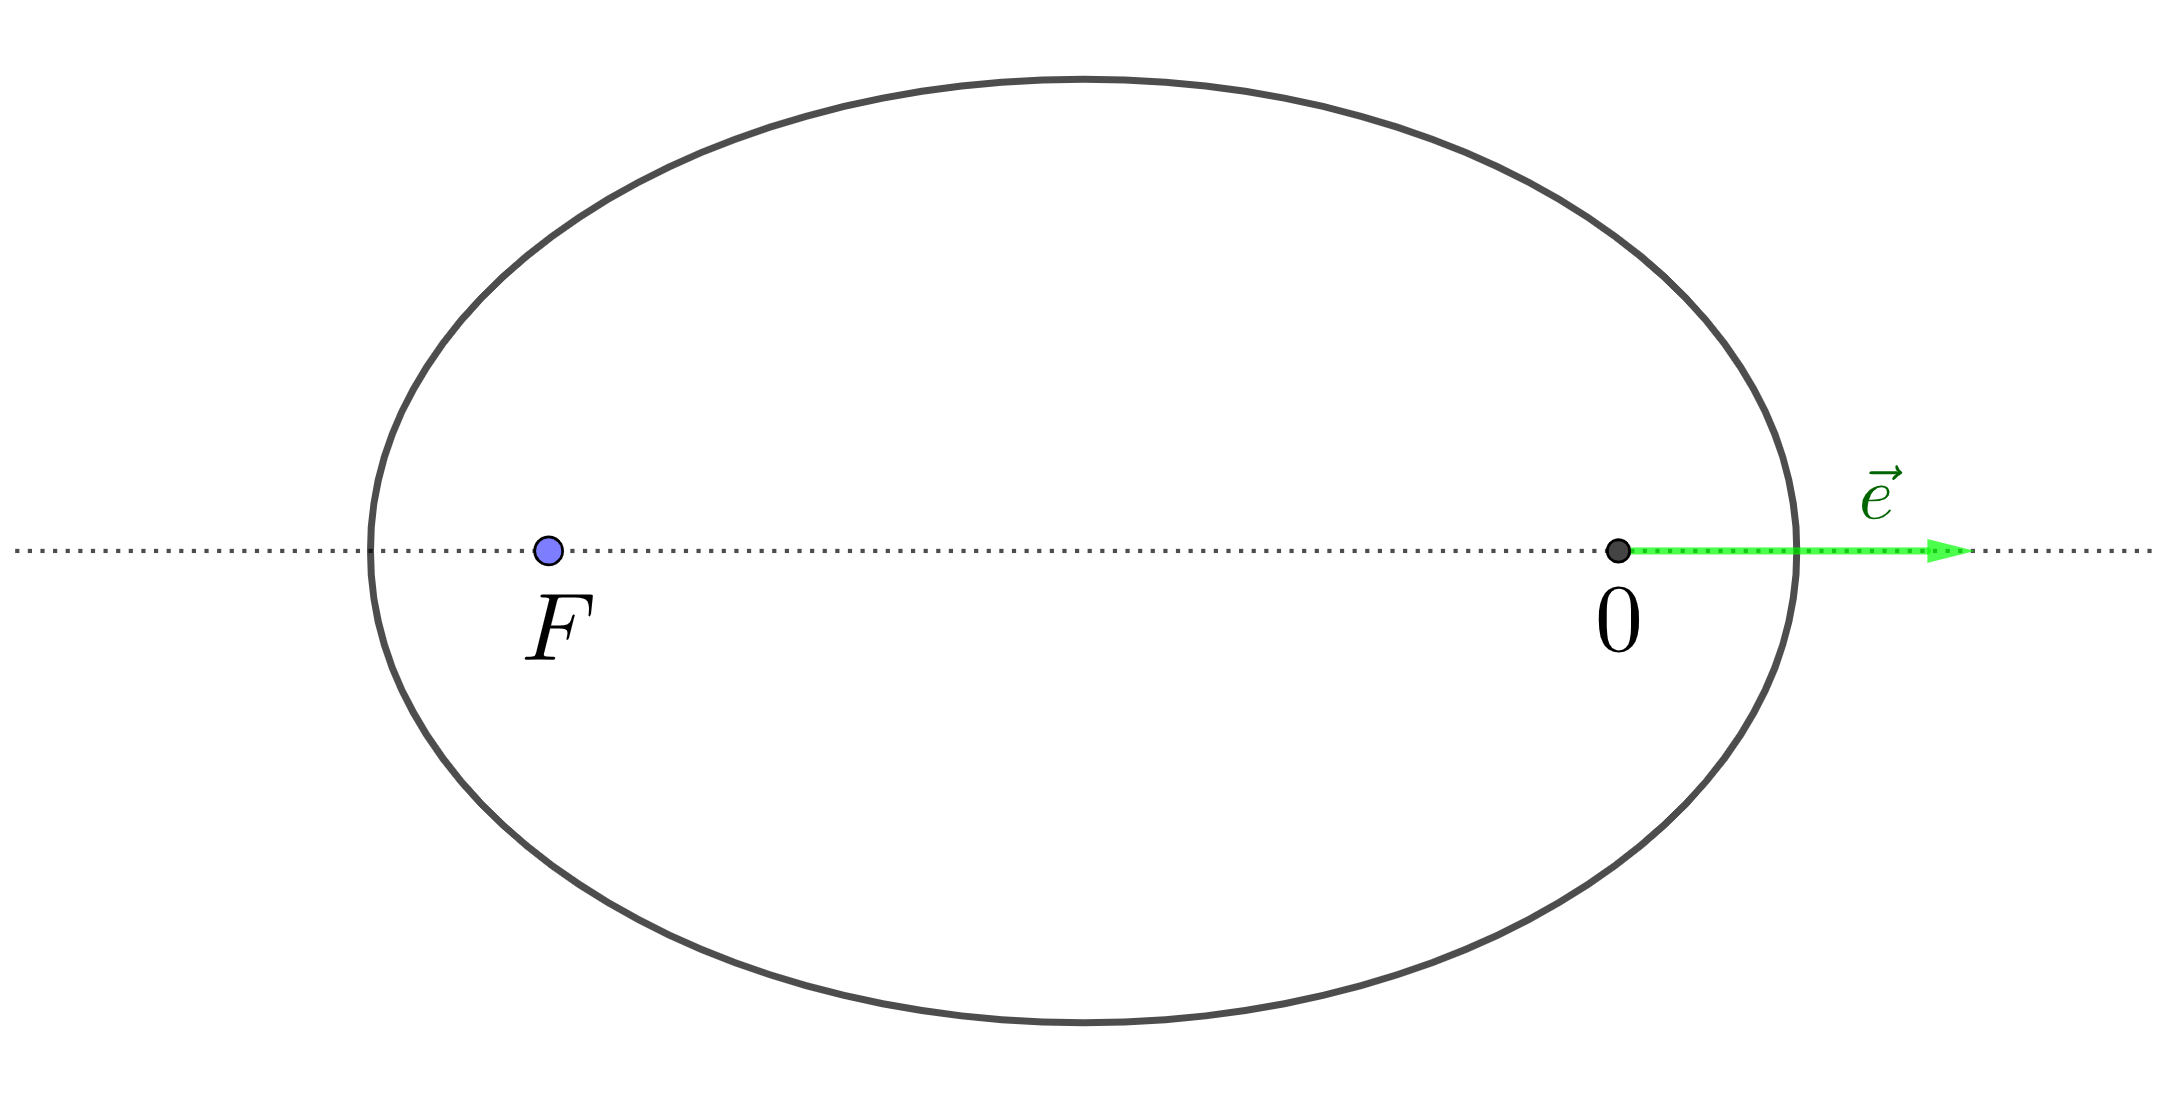
\includegraphics[scale=0.1]{images/elipse_excentricidad.png}
\caption{Representación de una elipse junto a sus focos y el vector $\vec{e}$.}
\label{fig:elipse_excentricidad}
\end{figure}

Llamaremos a $|\vec{e}|=e$ la \textbf{excentricidad de la elipse}, tomando valores en $[0,1[$. A mayor valor de excentricidad, mayor separación entre los focos, y viceversa. Si el valor de $e$ es 1, la órbita del objeto es una parábola, y si es mayor que 1, el objeto describirá una órbita hiperbólica.\\

Si trazamos una recta que pase por los dos focos de nuestra elipse, como podemos ver en \hyperref[fig:elipse_excentricidad]{la figura \ref{fig:elipse_excentricidad}}, dicha recta se intersecará con la elipse, obteniendo así dos puntos a los que llamaremos perihelio ($P$, más cercano a $0$) y afelio ($A$, más cercano a $F$). Si tomamos el centro de la elipse como el punto medio entre los dos focos y medimos la distancia desde el centro hasta el perihelio, obtendremos el \textbf{semieje mayor} de la elipse, al que notaremos por $a$. Por otra parte, si trazamos una perpendicular a la recta que pasa por los focos que pase por el centro de la elipse, la distancia desde una de las intersecciones con la elipse hasta el centro nos dará el semieje menor, al que representaremos por $b$. Podemos entender más fácilmente estos valores en la siguiente figura.

\begin{figure}[H]
\centering
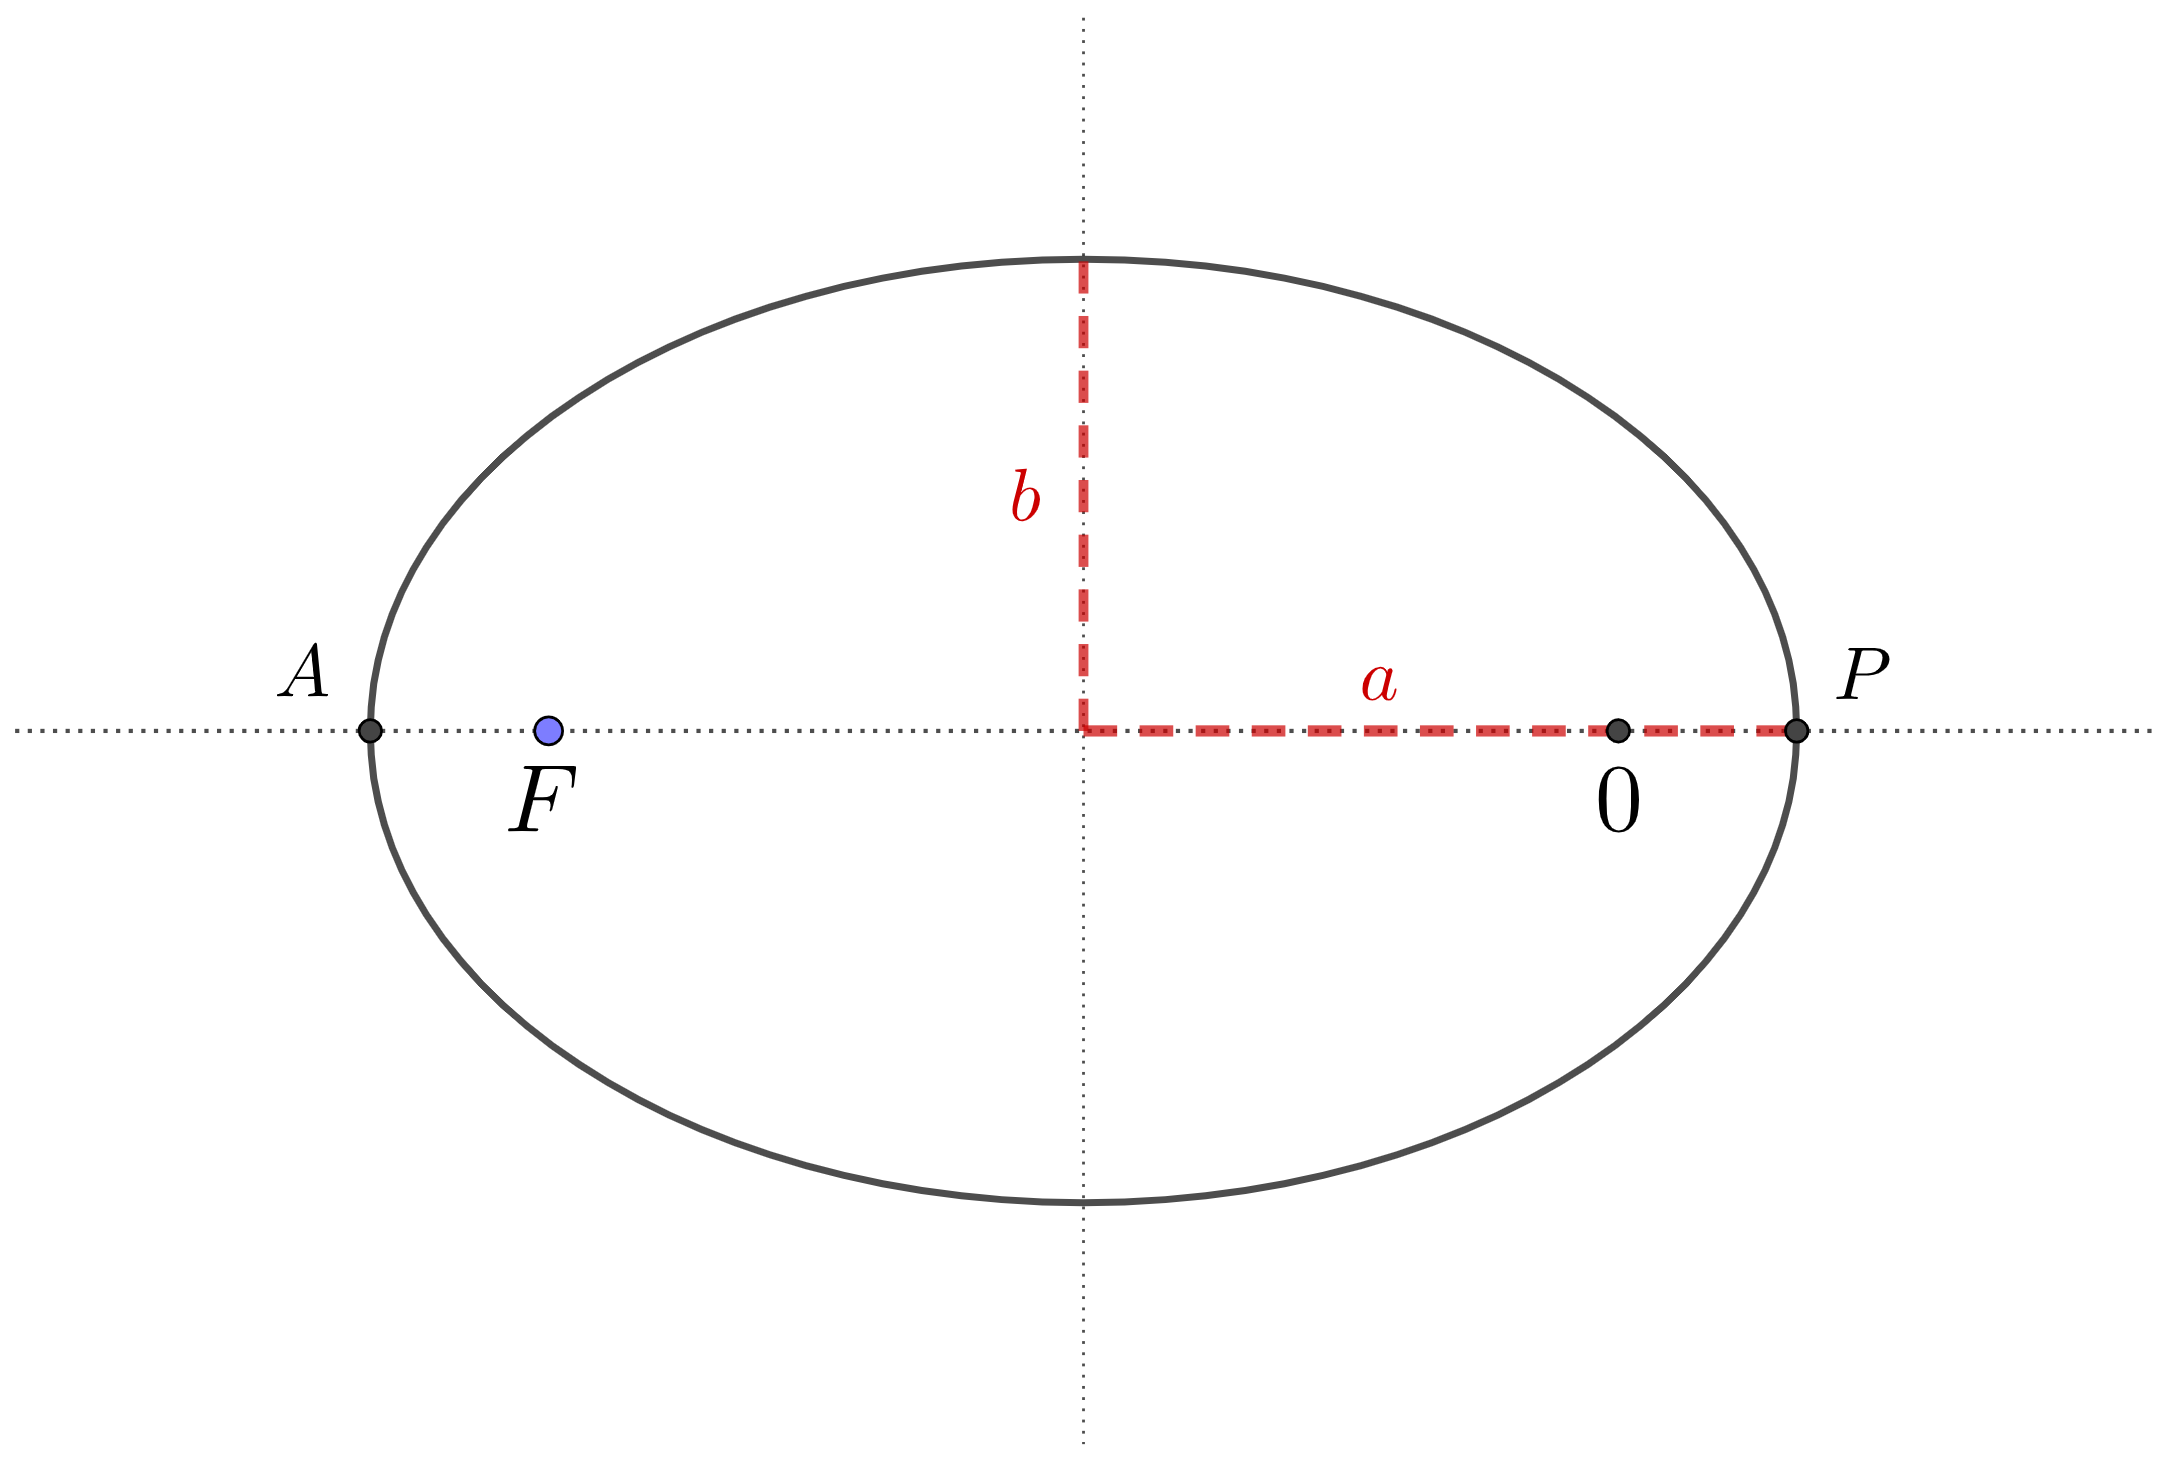
\includegraphics[scale=0.12]{images/perihelio_afelio.png}
\caption{Elementos geométricos de la elipse.}
\label{fig:perihelio_afelio}
\end{figure}

Notemos dos relaciones interesantes entre los elementos de la elipse comentados anteriormente y su excentridad, que mostramos a continuación:

\[
\frac{b}{a}=\sqrt{1-e^2}, \; \; \; \; \; \; \; \; \; \; \; \; \; \; \; \; \; \; \; \; e=\frac{\text{distancia entre los focos}}{\text{eje mayor}}=\frac{\overline{OF}}{2a}
\]\\

Por último, notemos por $\omega\in\mathbb{R}/2\pi\mathbb{Z}$ al \textbf{argumento del perihelio}, que representará el ángulo formado entre el eje polar (equivalente al eje $x$ en el sistema cartesiano) y la dirección del vector $\vec{e}$. Así, tenemos que:
\[
a=e(\cos{\omega},\sin{\omega})
\]

Llamemos $\mathcal{E}_0$ al espacio de elipses con foco en el origen, donde cada elipse queda determinada de manera única por su \hyperref[eq:elipse_cartesiana]{ecuación cartesiana}. Los parámetros $a$, $e$ y $\omega$ dan lugar a sistema de coordenadas en $\mathcal{E}_0$, que está definido sobre $\mathbb{R}^2$. Aquí surge un problema, pues las órbitas de los planetas son elipses en el espacio, cada una situada en un plano distinto, con un sentido de giro. Por tanto, será necesario definir un nuevo conjunto de parámetros para obtener un sistema de coordenadas sobre tres dimensiones.\\

Para empezar, definamos un sistema de referencia ortonormal en el espacio, que situará al Sol en el origen, y el plano $z=0$, en el que se encontrará el recorrido de la órbita de la Tierra, llamado plano de la eclíptica.\\

Empezamos definiendo el vector unitario $\vec{e}_1$ que tomamos en la recta que pasa por el sol con dirección la constelación de Aries, estrella fija que pertenece al plano de la eclíptica. El vector $\vec{e}_2$ lo definimos como el vector ortonormal a $\vec{e}_1$ que está también en el plano de la eclíptica. Como hay dos opciones, tomaremos el que da sentido positivo al giro de la Tierra (giro antihorario). Por último escogemos el vector $\vec{e}_3$ como el perpendicular unitario a los dos anteriores, y al tener de nuevo dos opciones, lo fijamos a partir de la orientación que da el eje terráqueo de Sur a Norte.\\

\begin{figure}[H]
\centering
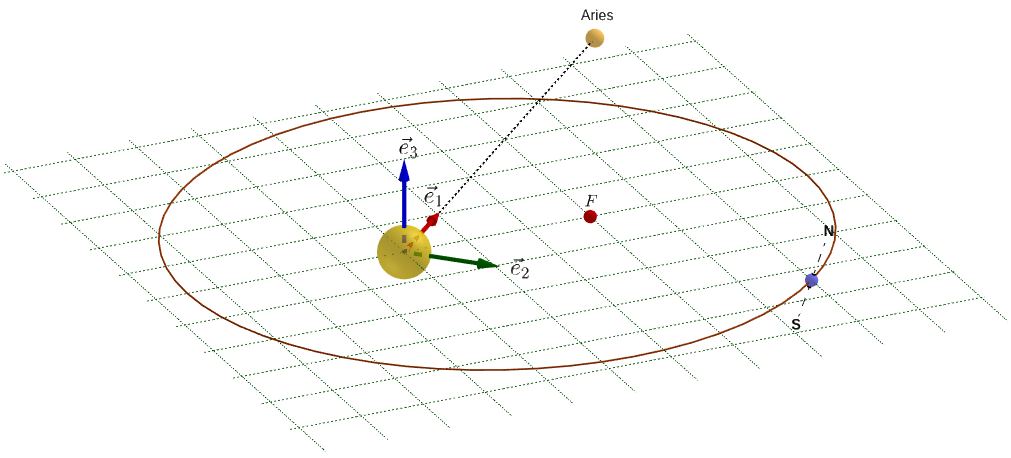
\includegraphics[scale=0.35]{images/sistema_referencia_1.png}
\caption{Órbita elíptica de la Tierra con focos $F$ y el Sol, mostrando el sistema de referencia. En la órbita terrestre real, el foco $F$ se encuentra dentro del Sol.}
\label{fig:sistema_referencia}
\end{figure}

Así, tenemos un sistema ortonormal $\{\vec{e}_1,\vec{e}_2,\vec{e}_3\}$ de manera que la orientación del movimiento de la Tierra se corresponde con la orientación $\{\vec{e}_1,\vec{e}_2\}$ del plano de la eclíptica.\\

Para determinar una órbita elíptica por completo necesitaremos cinco elementos; $a$, $e$ y $\omega$ definidos anteriormente, y dos más que introduciremos a continuación que definirán el plano de movimiento: la inclinación respecto al plano de la eclíptica ($i$) y el argumento del nodo ascendente ($\Omega$).\\

Fijemos la línea de nodos como la recta que interseca el plano de movimiento del objeto observado y el plano de la eclíptica; sean $\vec{n}$ el vector normal al plano de movimiento y $\mathcal{N}_+$ el lado positivo de la línea de nodos. Entonces:

\[
\left\{
\begin{array}{l}
	i=\measuredangle(\vec{e}_3,\vec{n}), \; \; \; \; \; \; \; \; \; \; i\in]0,\pi[\\
	\Omega=\measuredangle(\vec{e}_1, \mathcal{N}_+), \; \; \; \; \; \Omega\in\mathbb{R}/2\pi\mathbb{Z}
\end{array}
\right.
\]\\

Una vez hayamos definido el plano de movimiento con estos dos valores, encontramos la elipse usando la línea de nodos como eje de rotación para el argumento del perihelio, $\omega$.

\begin{figure}[H]
\centering
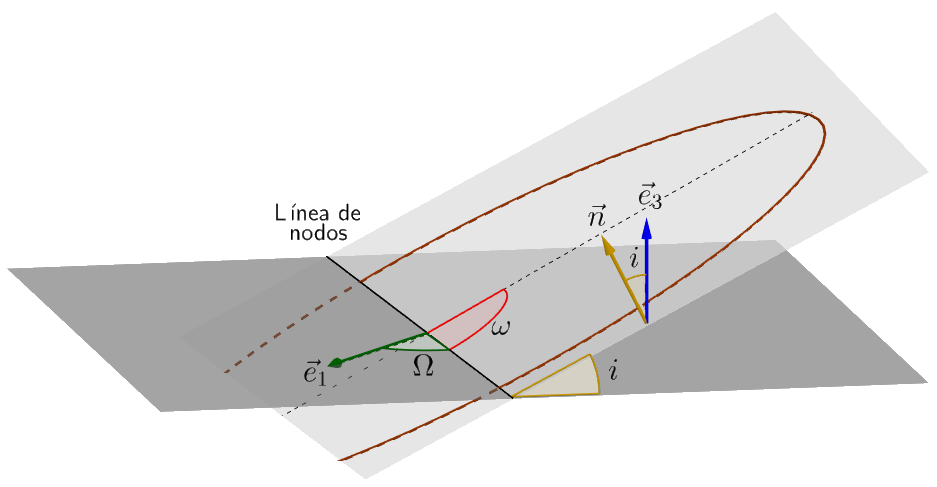
\includegraphics[scale=0.375]{images/omega_i_5.png}
\caption{Plano de movimiento definido por la inclinación y el argumento del nodo ascendente.}
\label{fig:omega_i}
\end{figure}

Al conjunto de estas cinco coordenadas lo llamaremos coordenadas astronómicas, y están bien definidas y son unívocas en la región $i\in]0,\pi[$, $e\in]0,1[$, excluyendo así las órbitas circulares y las definidas sobre el plano de la eclíptica.\\

Para terminar, definamos el valor $T$ como el momento de paso por el perihelio, la fecha concreta del momento en el que el objeto está en el perihelio de su órbita después del 31 de diciembre de 1899 (\textit{creo que esto no es exactamente así}), que definirá, junto al resto de elementos, la posición del cuerpo en su órbita en cualquier momento.\\

\noindent \textit{Seguramente sea buen idea hablar de como pasar el origen a la Tierra y pasar a coordenadas ecuatoriales geocéntricas. Moulton 185}\\


\subsection{Coordenadas Ecuatoriales}
Cada lugar en la Tierra puede ser localizado conociendo su latitud (ángulo en grados sobre el ecuador) y su longitud (ángulo en grados sobre el meridiano cero, el meridiano de Greenwich). De la misma manera, podemos definir ciertos valores para fijar la localización de todo objeto en la bóveda celeste, a los que llamaremos ascensión recta, $\alpha$, equivalente a la longitud, y declinación, $\delta$, equivalente a la latitud. \\

Al igual que utilizamos una localización física en la Tierra como referencia para la longitud, utilizaremos el equinoccio vernal (\textit{de primavera?}) como referencia para la ascensión recta, que se encontrará en el punto de la eclíptica donde el Sol pasa del hemisferio sur al hemisferio norte. A partir de la recta que une el centro de la Tierra con este punto se tomará el ángulo que forma con nuestro objeto observado. Para la declinación tomaremos el ecuador celeste, un gran círculo en la bóveda celeste en el mismo plano que el ecuador terrestre.\\

\begin{figure}[H]
\centering
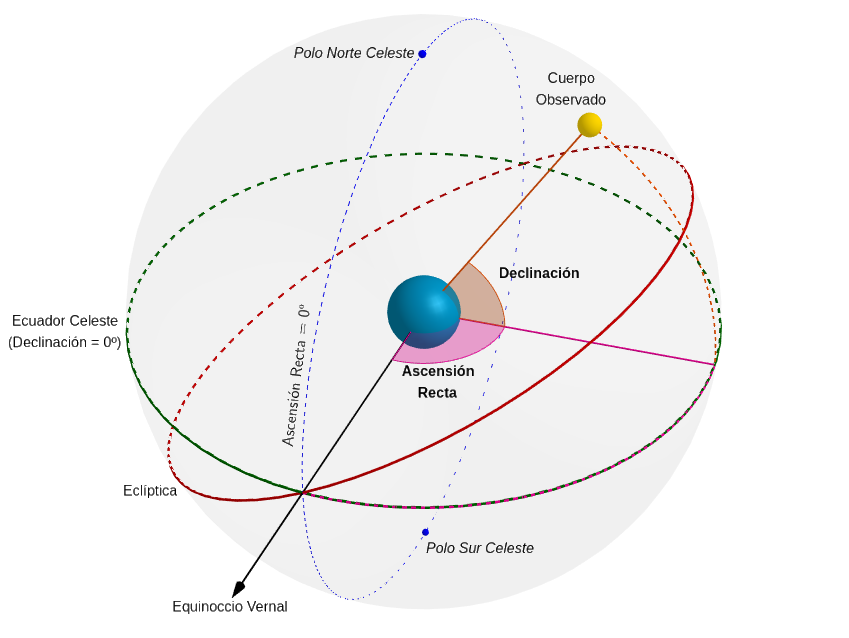
\includegraphics[scale=0.4]{images/ascension_declinacion.png}
\caption{La Tierra, en el centro, junto a la ascensión recta y declinación de cierto objeto. El círculo rojo define el camino aparente del Sol en el cielo, que define el plano de la eclíptica.}
\label{fig:ascension_declinacion}
\end{figure}

La declinación es medida en grados, como la latitud. Pero, a diferencia de la longitud, la ascensión recta es medida en horas, minutos y segundos en dirección este. Como en un día hay 24 horas, cada hora de ascensión recta corresponderá a una veinticuatroava parte de la rotación total de la Tierra, y por tanto, una hora será igual a $\frac{360}{24}=15º$.\\

Al conjunto de estas dos coordenadas se les llama Coordenadas Ecuatoriales, y junto a una distancia dada podremos definir la posición exacta de un objeto en cierto momento.\\


\section{Caminos e ideas para desarrollar el método de determinación}

\textit{No estoy contento con el título de la sección, me gustaria poner algo para representar que aquí se habla de cómo Gauss y Lagrange llegan a la idea principal para desarrollar su método}\\

Una vez obtenidas las coordenadas ecuatoriales de un objeto mediante tres observaciones, las podemos escribir como un grupo de funciones de los elementos orbitales del cuerpo en el momento de las observaciones, $t_1, t_2, t_3$. Así, obtenemos lo siguiente:
\begin{align}
\left\{\begin{array}{l}
	\alpha_1 = \phi(a, e, \omega, i, \Omega, T; t_1)\\ 
	\alpha_2 = \phi(a, e, \omega, i, \Omega, T; t_2)\\ 
	\alpha_3 = \phi(a, e, \omega, i, \Omega, T; t_3)\\ 
	\delta_1 = \psi(a, e, \omega, i, \Omega, T; t_1)\\ 
	\delta_2 = \psi(a, e, \omega, i, \Omega, T; t_2)\\
	\delta_3 = \psi(a, e, \omega, i, \Omega, T; t_3)
\end{array}
\right.
\label{eq:ascension_declinacion}
\end{align}

\noindent donde:

\begin{itemize}
\item $\phi$ y $\psi$ son la ascensión recta y declinación, funciones de los elementos de la órbita y el momento de la observación.
\item $a$ es el semieje mayor de la órbita.
\item $e$ es la excentricidad de la órbita.
\item $\omega$ es el ángulo respecto al eje de excentricidad.
\item $i$ es el ángulo de inclinación.
\item $\Omega$ es la longitud del nodo ascendente.
\item $T$ es el momento de paso por el perihelio.
\end{itemize}

Pues bien, el problema de determinación de órbitas consistirá en resolver todas estas ecuaciones para los seis elementos desconocidos, pero, las funciones de ascensión recta y declinación involucran a los elementos muy enrevesadamente, además de que son altamente trascendentales.\\

La órbita a determinar podrá ser una elipse, una hipérbola o una parábola. Para el primer caso, encontraremos la posición de la órbita utilizando la ecuación de Kepler (\textit{hablar sobre esto en algún punto}), y de manera similar para el segundo caso. Por otra parte, si la órbita es una parábola, hemos de utilizar una ecuación cúbica. Por tanto, ya que en los tres casos las coordenadas se obtienen mediante una serie de transformaciones trigonométricas, no dispondremos de soluciones directas para estas ecuaciones mediante métodos ordinarios.\\

\textit{(Aquí puede que ponga algo más)}\\

Volvamos a las \hyperref[eq:ascension_declinacion]{ecuaciones \ref{eq:ascension_declinacion}}, y supongamos que queremos las coordenadas polares y sus derivadas, por ejemplo, en $t=t_2$. Estas ecuaciones cambian a:
\begin{align}
\left\{\begin{array}{l}
	\alpha_1 = f(\alpha_2, \delta_2, \rho_2, \alpha_2', \delta_2', \rho_2'; t_1, t_2)\\ 
	\alpha_2 = \alpha_2\\
	\alpha_3 = f(\alpha_2, \delta_2, \rho_2, \alpha_2', \delta_2', \rho_2'; t_2, t_3)\\
	\delta_1 = g(\alpha_2, \delta_2, \rho_2, \alpha_2', \delta_2', \rho_2'; t_1, t_2)\\
	\delta_2 = \delta_2\\
	\delta_3 = g(\alpha_2, \delta_2, \rho_2, \alpha_2', \delta_2', \rho_2'; t_2, t_3)
\end{array}
\right.
\label{eq:idea_laplace}
\end{align}

\noindent donde $\rho$ es la distancia al origen en $t_2$ y:
\[
\alpha_2'=\frac{d\alpha}{dt}, \; \; \; \delta_2'=\frac{d\delta}{dt}, \; \; \; \rho_2'=\frac{d\rho}{dt} \; \; \;  \text{en} \; \; t=t_2
\]

Así, solo tendremos que resolver cuatro ecuaciones para cuatro incógnitas, pues $\alpha_2$ y $\delta_2$ son conocidas. Pero, además, podemos modificar estas ecuaciones para hacer que sean más fáciles de determinar, y de esta manera aparece el método de \textbf{Laplace}, que fue desarrollado y aplicado por primera vez para determinar una órbita en 1780.\\

Por otra parte, podemos tomar tres coordenadas en dos momentos diferentes, $t_1$ y $t_3$, para así obtener otro conjunto de elementos a determinar, y haciéndonos así con dos ecuaciones con solamente dos incógnitas, que podrán ser resueltas.
\begin{align}
\left\{\begin{array}{l}
	\alpha_1 = \alpha_1\\
	\alpha_2 = F(\alpha_1, \delta_1, \rho_1, \alpha_3, \delta_3, \rho_3; t_1, t_2, t_3\\
	\alpha_3 = \alpha_3\\
	\delta_1 = \delta_1\\
	\delta_2 = G(\alpha_1, \delta_1, \rho_1, \alpha_3, \delta_3, \rho_3; t_1, t_2, t_3)\\
	\delta_3 = \delta_3
\end{array}
\right.
\label{eq:camino_gauss}
\end{align}

Este es el camino que siguió Lagrange para resolver el problema en 1778, y que retomó \textbf{Gauss} en 1801.\\

A pesar de la cantidad de estudios que se han realizado tras la publicación de estos métodos, muy poco de lo que es realmente nuevo o teóricamente importante se ha añadido a las determinaciones que desarrollaron Laplace y Gauss, a menos que se usen más de tres observaciones.\\


\section{Preparación y Corrección de las Observaciones}
Independientemente del método que queramos seguir para determinar la órbita del objeto observado, habremos de realizar algunas correcciones en los datos obtenidos antes de comenzar a realizar cálculos.\\

Debido a la protuberancia de la Tierra en el ecuador, la Luna y el Sol causarán una ligera oscilación periódica y un lento cambio secular en la posición del plano de su ecuador (\textit{frase muy parecida a la que aparece en Moulton página 194}). Así, en los dos equinoccios, en los que el ecuador y la eclíptica se intersecan, habrá pequeñas oscilaciones periódicas (nutación) y lentos cambios de la posición de la Tierra a lo largo de la eclíptica (precesión). En este caso, se acostumbra a utilizar el equinoccio medio (equinoccio prescindiendo de la nutación) y la posición del ecuador al comienzo del año en el que se estén haciendo las observaciones.\\

Por otra parte, la observación del objeto cuya órbita determinar también puede ser afectada por la aberración de la luz, es decir, la diferencia entre la posición observada del objeto y su posición real, causada por la combinación de la velocidad del observador (por la rotación de la Tierra) y la velocidad de la luz. Tendremos que corregir dos aberraciones: la anual, debida a la rotación de la Tierra alrededor del Sol, y la aberración diurna, debida a la rotación de la Tierra sobre su eje. Aún así, debido a que la velocidad de rotación es muy pequeña en comparación con la velocidad de traslación, la aberración diurna será relativamente pequeña, y podrá ser obviada, especialmente en el caso de que las observaciones tomadas no sea demasiado precisas.\\

Definamos como $\alpha_0$ y $\delta_0$ la ascensión recta y declinación del cuerpo observado en cierto momento. Entonces, sus valores referidos al equinoccio medio del comienzo del año, y corregidos para la aberración lumínica anual, son:
\[
\left\{
\begin{array}{l}
	\alpha = \alpha_0 - 15f - g \sin(G+\alpha_0) \tan(\delta_0) - h \sin(H+\alpha_0) \sec(\delta_0)\\
	\delta = \delta_0 - i \cos(\delta_0) - g \cos(G+\alpha_0) - h \cos(H+\alpha_0) \sin(\delta_0)
\end{array}
\right.
\]

\noindent donde $f, g, h, G$ y $H$ son cantidades auxiliares, a las que llamaremos \textit{números interestelares independientes}, y cuyo valor aparece en el \textit{American Ephemeris and Nautical Almanac} para cada día del año. Notar que estas correcciones serán expresadas en segundos de arco, pues en esta unidad son dadas las cantidades tomadas de la efemérides.\\

Por último, tendremos que corregir la aberración diurna a través de las siguientes ecuaciones:
\[
\left\{
\begin{array}{l}
	\Delta \alpha = -0''.322 \cos(\phi) \cos(\theta - \alpha_0) \sec(\delta_0)\\
	\Delta \delta = -0''.322 \cos(\phi) \sin(\theta - \alpha_0) \sin(\delta_0)
\end{array}
\right.
\]

\noindent donde $\phi$ representará la latitud del observador y $\theta-\alpha_0$ representa el ángulo horario del objeto en el momento de la observación (\textit{???}). La primera corrección será pequeña mientras que $\delta_0$ no sea cercano a $\pm90º$, y la segunda no podrá exceder el valor de $0''.322$.\\

\textit{DUDAS: como se utilizan las dos correciones a la vez???? $0''.322$ se refiere a 0.322 segundos??}\\


\section{Argumentación General para la Determinación}
Los dos métodos que vamos a estudiar a continuación (Laplace y Gauss) siguen una estrategia similar, que expondremos a continuación. Para empezar, supongamos que solo disponemos de tres observaciones de nuestro objeto en tres momentos diferentes, $t_1, t_2, t_3$, de manera que conocemos la ascensión recta y declinación en cada uno de estos instantes. A continuación, definamos algunos términos:
\begin{itemize}
\item Definimos $C$, $S$ y $E$ como el cuerpo observado, el Sol (alrededor del cual gira $C$) y la Tierra respectivamente.
\item Sean $(\xi,\eta,\zeta)$ las coordenadas (cartesianas) de $C$ respecto a $S$, $(X,Y,Z)$ las coordenadas de $S$ respecto a $E$, $(x,y,z)$ coordenadas de $C$.
\item $\rho$ es la distancia de $E$ a $C$, $r$ la distancia de $S$ a $C$ y $R$ la distancia de $E$ a $S$.
\end{itemize}

\begin{figure}[H]
\centering
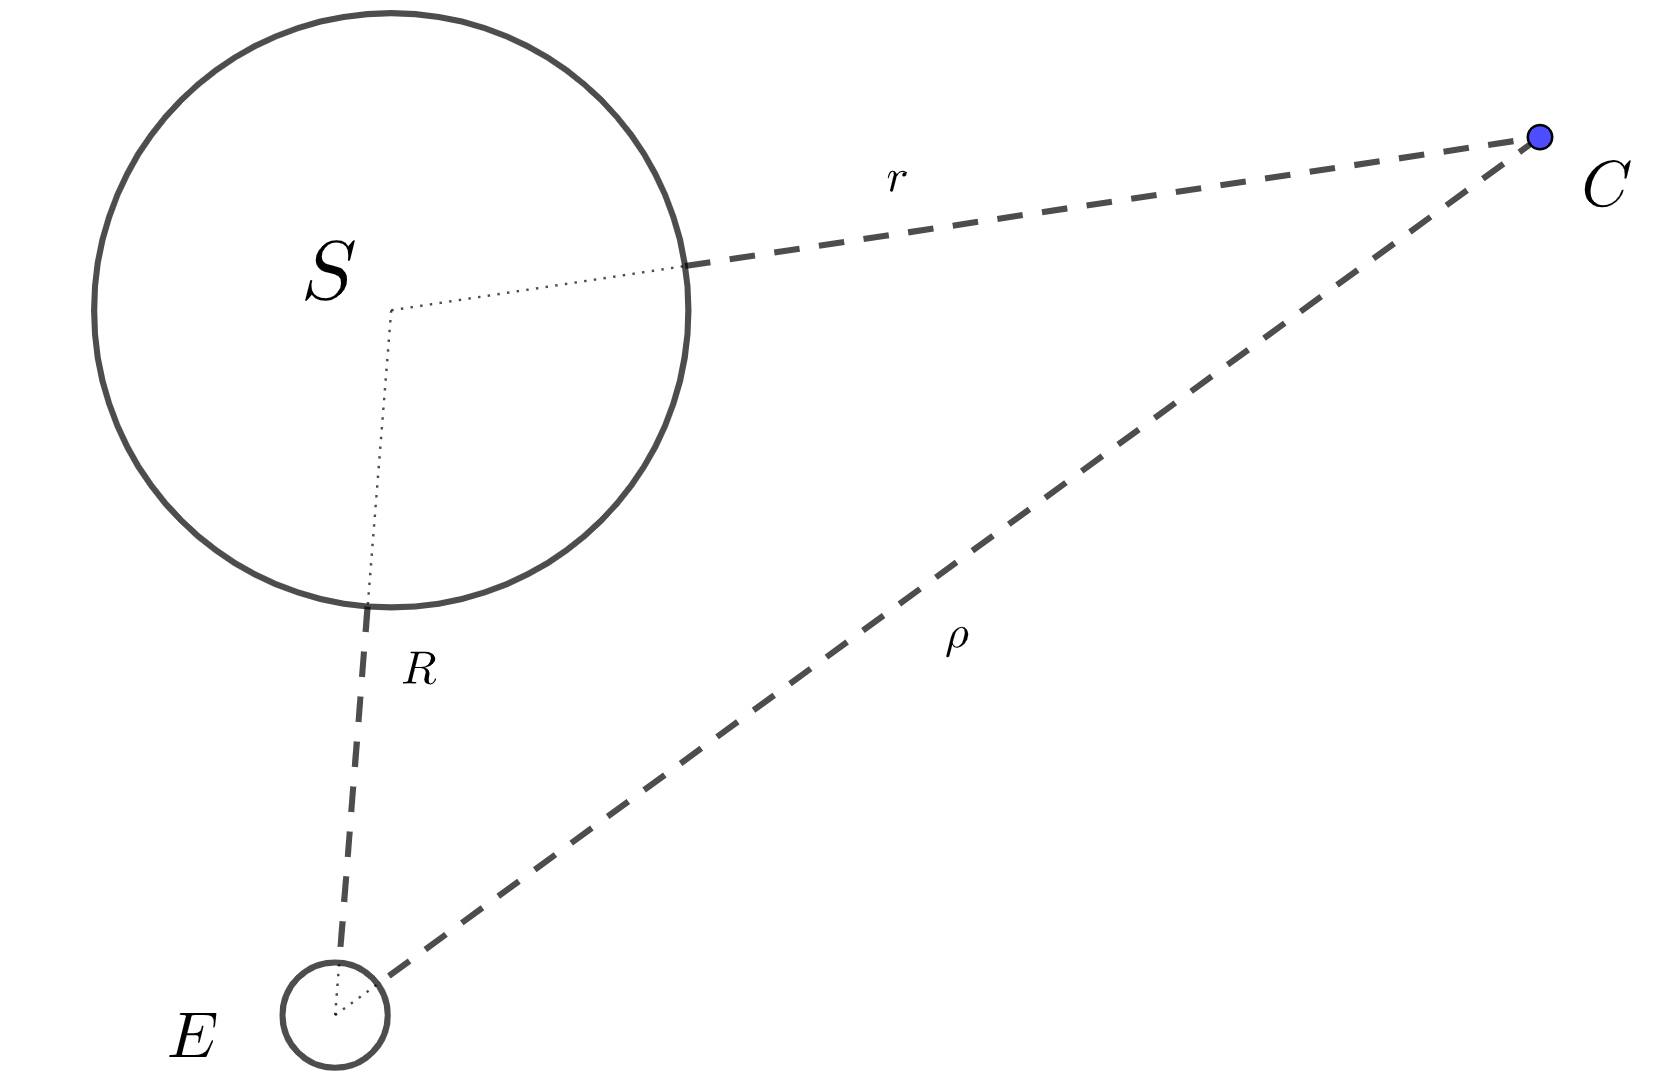
\includegraphics[scale=0.15]{images/notation.png}
\caption{Notación utilizada para nuestro problema}
\label{fig:notation}
\end{figure}

Con todo esto, podemos escribir:
\begin{align}
\left\{
\begin{array}{l}
\xi = \rho \cos{\delta}\cos{\alpha} = \rho\lambda\\
\eta = \rho \cos{\delta}\sin{\alpha} = \rho\mu\\
\zeta = \rho \sin{\delta} = \rho\nu
\end{array}
\right.
\label{eq:terminologia}
\end{align}

Ya que conocemos el valor de $\alpha$ y $\delta$ en $t_1$, $t_2$ y $t_3$, también conoceremos el valor en dichos momentos de $\lambda, \mu$ y $\nu$, que son los cosenos directores del vector que va de $E$ a $C$. Por tanto, habremos de determinar la distancia $\rho$.\\










\iffalse



\section{Método Gaussiano de Determinación}
Al igual que en el método de Laplace, volvamos a separar nuestro trabajo en distintos pasos.\\

\subsection{\normalfont{\textit{Imponer que $C$ se mueve en un plano que pasa a través de $S$}}}
Ya que $S$ es el origen de las coordenadas $x$, $y$ y $z$, podemos escribir la condición del enunciado como:
\[
\left\{
\begin{array}{l}
	Ax_1+By_1+Cz_1=0\\
	Ax_2+By_2+Cz_2=0\\
	Ax_3+By_3+Cz_3=0
\end{array}
\right.
\]

\noindent donde $A$, $B$ y $C$ son las constantes que determinan la posición del plano de movimiento. Eliminando estas incógnitas constantes llegaremos a:
\[
\left|
\begin{array}{ccc}
	x_1 & y_1 & z_1\\
	x_2 & y_2 & z_2\\
	x_3 & y_3 & z_3
\end{array}
\right|
=0
\]

A partir de este determinante podemos obtener tres ecuaciones expandiéndolo respecto a los elementos de las tres columnas, donde estas tres ecuaciones no serán más que diferentes formas de la misma. Aún así, si se determinen los paréntesis y las variables $x_i$, $y_i$ y $z_i$ se expresan en términos de coordenadas geocéntricas, obtendremos tres ecuaciones con las incógnitas $\rho_1$, $\rho_2$ y $\rho_3$.
\[
\left\{
\begin{array}{l}
	(y_2z_3-z_2y_3)x_1-(y_1z_3-z_1y_3)x_2+(y_1z_2-z_1y_2)x_3=0\\
	(x_2z_3-z_2x_3)y_1-(x_1z_3-z_1x_3)y_2+(x_1z_2-z_1x_2)y_3=0\\
	(x_2y_3-y_2x_3)z_1-(x_1y_3-y_1x_3)z_2+(x_1y_2-y_1x_2)z_3=0
\end{array}
\right.
\]\\

Los valores entre paréntesis representan las proyecciones de dos de los triángulos formados por $S$ y las posiciones de $C$ tomadas de dos en dos sobre los tres planos fundamentales. Por tanto, como en cada ecuación las tres áreas son proyectadas sobre el mismo plano (\textit{tengo que hacer algún dibujito de esto}), podremos utilizar los triángulos por si mismos en vez de sus proyecciones. Ahora, definamos $[1,2]$, $[1,3]$ y $[2,3]$ los triángulos formados por $S$ y $C$ en los momentos $t_1$, $t_2$ y $t_3$; con esto, las ecuaciones anteriores pasan a ser:
\[
\left\{
\begin{array}{l}
	[2,3]x_1-[1,3]x_2+[1,2]x_3=0\\
	{[2,3]}y_1-[1,3]y_2+[1,2]y_3=0\\
	{[2,3]}z_1-[1,3]z_2+[1,2]z_3=0
\end{array}
\right.
\]\\

\subsection{\normalfont{\textit{Desarrollar las relaciones entre los triángulos como series de potencias en los intervalos de tiempo}}}
Para resolver este paso, integraremos las \hyperref[eq:ley_gracitacion_C]{ecuaciones de la ley de gravitación} para $C$ como serie de potencias en los intervalos de tiempo de los que disponemos, y tras ello sustituiremos los resultados por $t=t_1,t_2,t_3$ en los coeficientes de las ecuaciones vistas en el paso anterior.\\

Para facilitar la escritura de estas series de potencias, comencemos definiendo los siguientes valores:
\[
\left\{
\begin{array}{l}
	k(t_2-t_1)=\theta_3\\
	k(t_3-t_2)=\theta_1\\
	k(t_3-t_1)=\theta_2\\
	\theta_2=\theta_1+\theta_3
\end{array}
\right.
\]

Con esta notación, la proporción entre los triángulos definidos anteriormente será:
\[
\left\{
\begin{array}{l}
	\frac{[2,3]}{[1,3]}=\frac{\theta_1}{\theta_2}[1+\frac{1}{6}\frac{\theta_2^2-\theta_1^2}{r_2^3}+...]\\
	\frac{[1,2]}{[1,3]}=\frac{\theta_3}{\theta_2}[1+\frac{1}{6}\frac{\theta_2^2-\theta_3^2}{r_2^3}+...]
\end{array}
\right.
\]\\

\subsection{\normalfont{\textit{Desarrollar las ecuaciones para determinar $\rho_1$, $\rho_2$ y $\rho_3$}}}
Utilizando la proporción entre los triángulos, las ecuaciones con los triángulos $[i,j]$ y \hyperref[eq:relacion_C_S_E]{esta ecuación} obtenemos lo siguiente:
\[
\left\{
\begin{array}{l}
	\theta_1[1+\frac{1}{6}\frac{\theta_2^2-\theta_1^2}{r_2^3}+...] (\lambda_1\rho_1-X_1)-\theta_2(\lambda_2\rho_2-X_2)+\\ \; \; \; \; \; \; \; \; \; \; \; \; \; \; \; \; \; \; \; \; \; \; \; \; \; \; \; \; \; +\theta_3[1+\frac{1}{6}\frac{\theta_2^2-\theta_3^2}{r_2^3}+...] (\lambda_3\rho_3-X_3)=0\\

	\theta_1[1+\frac{1}{6}\frac{\theta_2^2-\theta_1^2}{r_2^3}+...] (\mu_1\rho_1-Y_1)-\theta_2(\mu_2\rho_2-Y_2)+\\ \; \; \; \; \; \; \; \; \; \; \; \; \; \; \; \; \; \; \; \; \; \; \; \; \; \; \; \; \; +\theta_3[1+\frac{1}{6}\frac{\theta_2^2-\theta_3^2}{r_2^3}+...] (\mu_3\rho_3-Y_3)=0\\

	\theta_1[1+\frac{1}{6}\frac{\theta_2^2-\theta_1^2}{r_2^3}+...] (\nu_1\rho_1-Z_1)-\theta_2(\nu_2\rho_2-Z_2)+\\ \; \; \; \; \; \; \; \; \; \; \; \; \; \; \; \; \; \; \; \; \; \; \; \; \; \; \; \; \; +\theta_3[1+\frac{1}{6}\frac{\theta_2^2-\theta_3^2}{r_2^3}+...] (\nu_3\rho_3-Z_3)=0
\end{array}
\right.
\]\\

Las incógnitas que aparecen en estas ecuaciones son $\rho_1$, $\rho_2$, $\rho_3$ y $r_2$. Ya que esta última solo aparece al multiplicando por $\theta_1$, $\theta_2$ o $\theta_3$, podríamos suponer que en una primera aproximación que estos términos se pueden omitir, pudiendo obtener así los $\rho_i$ mediante ecuaciones lineales; sin embargo, tras un discusión sobre los determinantes que intervienen (\textit{buscar info}), llegamos al hecho de que será necesario mantener los términos en $r_2$ incluso en la primera aproximación.\\

La solución de las ecuaciones anteriores para $\rho_2$ tiene la forma:
\[
\Delta\rho_2=P+\frac{Q}{r_2^3},
\]

\noindent donde $\Delta$ será el determinante formado por los coeficientes de las incógnitas de $\rho_i$, y $P$ y $Q$ serán funciones de los valores $\lambda_i$, $\mu_i$, $\nu_i$, $X_i$, $Y_i$, $Z_i$ para $i=1,2,3$.\\

En cualquier instante $t_i$, $E$, $S$ y $C$ formarán un triángulo. Si tomamos $i=2$, los valores de $\rho_2$ y $r_2$ satisfarán la ecuación:
\[
r_2^2=\rho_2^2+R_2^2-2\rho_2R_2\cos{\psi_2}
\]

Con el valor de $\rho_2$ y $r_2$ determinado, tenemos que la solución para $\rho_1$ y $\rho_3$ para dos ecuaciones cualesquiera de las del principio es:
\[
\left\{
\begin{array}{l}
	M\rho_1=P_1\rho_2[1-\frac{1}{6}\frac{\theta_2^2-\theta_1^2}{r_2^3}+...]+Q_1\\
	M\rho_3=P_3\rho_2[1-\frac{1}{6}\frac{\theta_2^2-\theta_3^2}{r_2^3}+...]+Q_3
\end{array}
\right.
\]

\noindent donde $M$, $P_1$ y $P_3$ son funciones de valores ya conocido y $Q_1$ y $Q_3$ solo involucrarán la incógnita $r_2$, que ya ha podido ser calculada.\\

\subsection{\normalfont{\textit{Determinar $\rho_1$ y $\rho_3$}}}
Notar que el cálculo de $\rho_2$ y $r_2$ realizado anteriormente es exactamente lo mismo que el tercer paso del método de Laplace. Por tanto, solo bastará calcular $\rho_1$ y $\rho_3$ con la última ecuación que hemos visto en el paso anterior.\\

\subsection{\normalfont{\textit{Determinar los elementos de la órbita a partir de las posiciones conocidas de $C$ en los momentos $t_1$ y $t_3$}}}
Estas dos posiciones y la de $C$ definirán el plano de la órbita sin mucho más trabajo. En su desarrollo, Gauss resolvió el problema de determinación de los elementos restantes mediante dos ecuaciones que solo involucraban las dos incógnitas. Una de ellas se obtiene de la proporción del triángulo formado por $S$, $E$ y $C$ en $t_1$ y $t_3$ con el área comprendida entre $r_1$, $r_3$ y el arco de la órbita descrito en el intervalo $[t_1,t_3]$; la otra ecuación deriva de la ecuación de Kepler en los momentos $t_1$ y $t_3$.\\

Aunque estas fórmulas sean complejas, el método de resolución para cada una de ellas es un proceso rápido de aproximaciones sucesivas, y tras resolver estas ecuaciones los elementos son de terminados fácilmente de manera única.\\
\fi










\newpage

\begin{thebibliography}{99}
\bibitem{moulton} \textsc{Forest Ray Moulton}, \textsc{An Introduction to Celestial Mechanics}, \textit{second edition}.

\bibitem{ortega} \textsc{R. Ortega, A.J. Ureña}, \textsc{Introducción a la Mecánica Celeste}.

\bibitem{right_ascension_declination} \textsc{Sky \& Telescope}, \textsc{Right Ascension and Declination: Celestial Coordinates For Beginners}, \url{https://skyandtelescope.org/astronomy-resources/right-ascension-declination-celestial-coordinates/}

\end{thebibliography}

\end{document}
